\section{Functionality}

In order to implement the functionalities of the concepts described in the previous section, editors are needed. Each of these editors will be described in this section.

\subsection{Petri net Editor}

\subsubsection{Purpose}
The basis for the main functionality of the software is the Petri net Editor. This editor enables a user to create or edit a Petri net that can be interpreted and used by the other editors. 

\subsubsection{Users}
Users with knowledge of Petri net logic and general technical skills are the main users of the Petri net editor. However, both simple and complex Petri nets can be implemented, so the technical skills of the users may vary accordingly. 


\subsubsection{Use cases}
The main use cases of the Petri net Editor are conveyed in the following diagram:

\begin{figure}[htp]
\begin{center}
  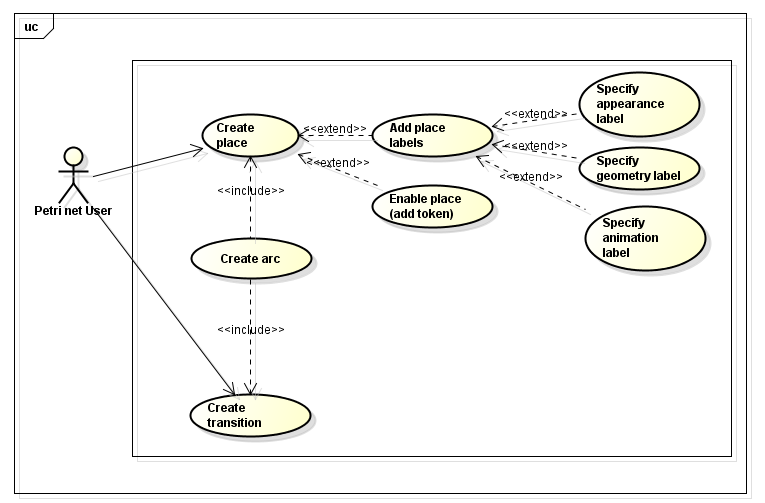
\includegraphics[width=0.8\textwidth]{image/PetrinetUC.png}
  \caption{Use cases for the Petri net Editor}
  \label{fig:petrinet_editor_usecases}
\end{center}
\end{figure}


The user will be able to create places, arcs and transitions. The user must start by creating a place or transition, arcs can only be created once there is a target and a source. A place or a transition can be dragged from a menu to the canvas, while the arc must be selected in the menu, then dragged from the source to the target. The user will be able to make the arc bi-directional by dragging a new arc in the opposite direction of the existing. 

A place can have up to three labels associated: appearance, geometry and animation. These labels are used to control the appearance, geometry and animation in the simulator. 

An example of an appearance label is "train", which will tell the simulator to use the appearance linked to "train" for the token(s) and the arcs associated with the place. See "Appearance editor" Section \ref{sec:appearance}. An example of an animation label is "fast", which will enable a fast token movement on the place and associated arcs. An example of a geometry label is "line\_1", which will link the place to a line specified in the geometry editor. 

Finally, a user can enable a place to receive input during runtime; this will enable the user to add a token on that place.

The Petri net editor is linked to the other editors, especially through labels. In the following, the Geometry editor will be described. 

\subsection{Geometry editor}


\subsubsection{Purpose}
As it has been previously discussed in Section \ref{sec:overall}, in order to create a 3D representation of the Petri net model, we need to add some geometrical information to it.  For this purpose, the user will interact with a geometry editor to define the location of the objects defined by the Petri net editor. These objects on their location will later be displayed in the 3D visualisation model. 
The geometry editor will allow the user to:
\begin{itemize}
\item draw lines - corresponding to places in the Petri net model
\item add bend points to lines - for creating curved lines
\item draw connectors - corresponding to transitions in the Petri net model
\item add input points  - corresponding to special constraints for transitions (e.g switches, traffic lights, etc.)
\end{itemize}

\subsubsection{Users}
The geometry editor will be used by technical users who are familiar with basic geometrical concepts and have a clear vision on how a geometry model is designed. No other specific previous knowledge is required but comprehension of Petri net models is an advantage.
\subsubsection{Use cases}
The main use cases of the Geometry editor are displayed in the following diagram:

\begin{figure}[htp]
\begin{center}
  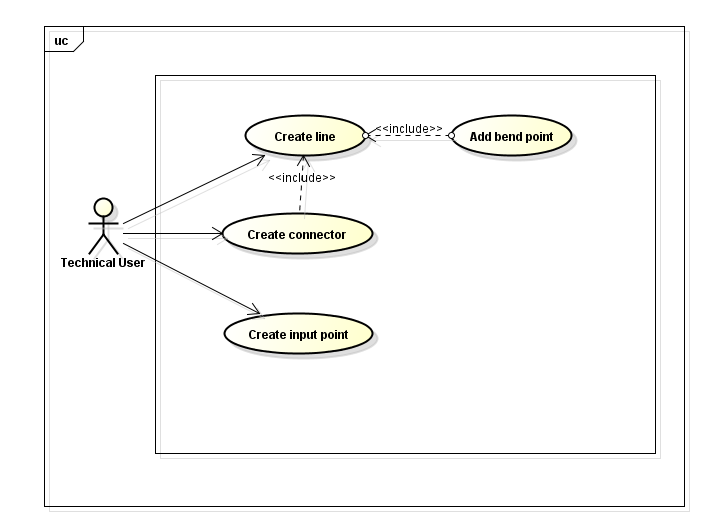
\includegraphics[width=0.8\textwidth]{image/GeometryUC.png}
  \caption{Use cases for the Geometry Editor}
  \label{fig:geometry_editor_usecases}
\end{center}
\end{figure}

\begin{enumerate}
	\item \textbf{Create line}: The user drags a line from the editor menu and draws it in the canvas. The number of lines is not restricted so the action can be repeated as many times as it is necessary but it is compulsory to have two connectors created before attempting to draw a line. Lines should also have a label that links back to the Petri net element it refers to.
	\item \textbf{Add bend point}: Bend points can only be added after a line has been created by clicking the line in order to create a curve. The number of bend points per line is restricted to one.
\item \textbf{Create connector}: Connectors can also be created from the editor menu and drawn in the editor window. Their functionality is to link two or more lines together. 
\item \textbf{Create input point}: Input points will be created in a similar way from the editor menu and can be placed anywhere in the canvas. However, they will have a label and an appearance attached to them in order to define the link back to the Petri net.   
\end{enumerate}

\subsection{Appearance Editor}
\subsubsection{Purpose}
The next step in reaching the 3D visualization of the Petri net model is to determine the visual characteristics for each element in the model. For this purpose, the appearance editor is used to define the shape, color, texture and any other information needed for a clear display of the initial model. 
\subsubsection{Users}
	The appearance editor can be used by any user both technical and nontechnical as it only implies linking the appearance labels defined in the Petri net model to a file containing all the information related to visual aspects: shape, texture, color. These can be .jpg files or special 3D documents whose structure is yet to be discussed.

\subsubsection{Use cases}
	The main use cases of the appearance editor are conveyed in the following diagram: 
	
	\begin{figure}[htp]
\begin{center}
  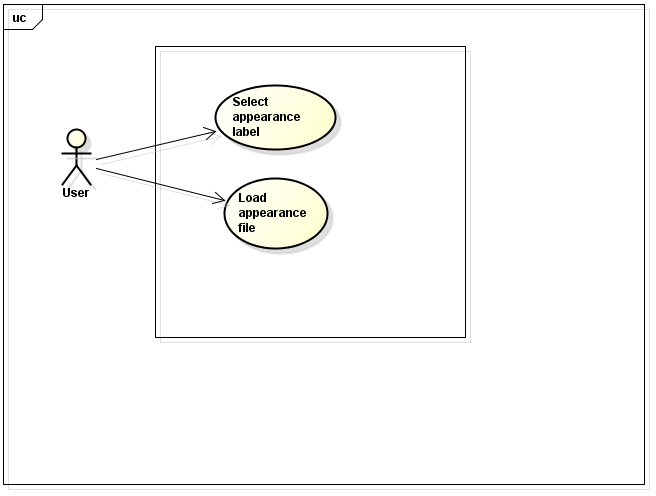
\includegraphics[width=0.8\textwidth]{image/AppearanceUC.png}
  \caption{Use cases for the Appearance Editor}
  \label{fig:appearance_editor_usecases}
\end{center}
\end{figure}


%\subsection{Use case description}

\begin{enumerate}
\item \textbf{Select appearance label}: The user will be able to select one of the appearance labels previously defined in the Petri net editor from a pop-up menu. For example, if the user wants to add appearance information to a token which in the Petri net model has as appearance label "train", then his/her selection from the pop-up menu should also be "train". The next step is described in use case 2. 
\item \textbf{Load appearance file}: The appearance editor will allow the user to browse among a list of files containing information related to the 3D visualization and load the one corresponding to the previously selected label.  
\end{enumerate}

   
 
\subsection{Configuration Editor}
\subsubsection{Purpose}
The configuration editor is intended to define a link between the Petri net model, the geometry and the appearance information files previously created by the user. Each element in the Petri net should have a corresponding geometry figure and appearance features assigned in order to have a valid configuration file for the simulation.   
\subsubsection{Users}
This editor will be used by all users, both technical and nontechnical as it only implies the association between three existing files. The interface should be intuitive and organised in a way that is familiar to the user in terms of loading files therefore no particular knowledge is required. 
\subsubsection{Use cases}
The main use cases for the configuration editor are conveyed in the following diagram: 

\begin{figure}[htp]
\begin{center}
  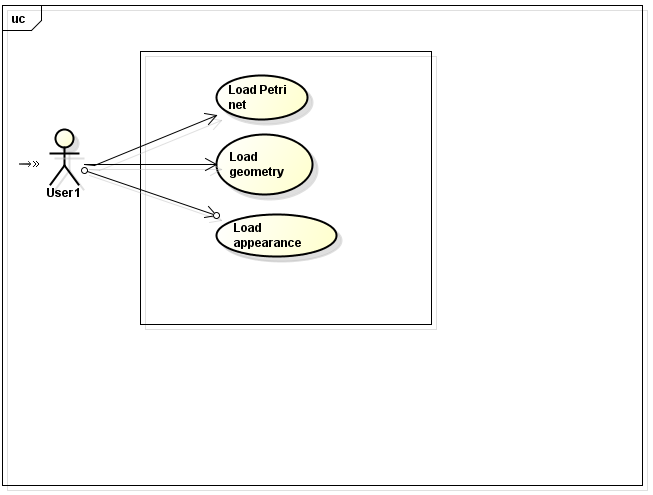
\includegraphics[width=0.6\textwidth]{image/ConfigurationUC.png}
  \caption{Use cases for the Configuration Editor}
  \label{fig:configuration_editor_usecases}
\end{center}
\end{figure}

\begin{enumerate}
\item \textbf{Load Petri net}: The user will be able to browse and load a Petri net model file designed using the Petri net Editor.
\item \textbf{Load geometry}: The user will be able to browse and load a geometry file designed using the Geometry Editor.
\item \textbf{Load appearance}: The user will be able to browse and load an appearance file designed using the Appearance Editor.
\end{enumerate}

\subsection{Simulator}
\subsubsection{Purpose}
Once the Petri net Editor and Geometry Editor have been set up correctly the user will be able to run the 3D simulation based on the information from the Appearance and Geometry Editor. During the 3D simulation the user will be able to add or remove trains, control traffic lights and control railroad switches through a Graphical User Interface (GUI).
\subsubsection{Users}
The simulator can be used by any user, both technical and nontechnical as they both have an interest in seeing the 3D visualization of the work done in the editors. Users do not need to have any prior knowledge about Petri nets since the simulation is controlled with a GUI and has no visual connection to the Petri net. 
\subsubsection{Use cases}
The main use cases for the Simulator are conveyed in the following diagram: 

\begin{figure}[htp]
\begin{center}
  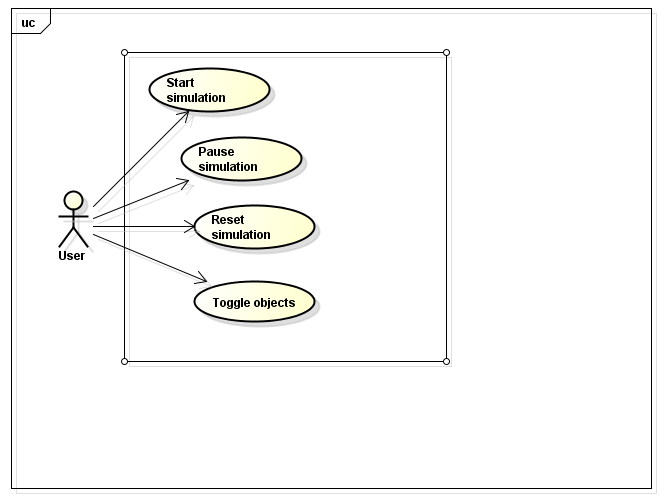
\includegraphics[width=0.8\textwidth]{image/SimulatorUC.png}
  \caption{Use cases for the Simulator}
  \label{fig:simulator_usecases}
\end{center}
\end{figure}

\begin{enumerate}
	\item \textbf{Start, pause and reset}: The user is able to start, pause and resume the simulation with 2 different buttons: one for play and pause, and another for resetting the simulation.
	
	\item \textbf{Toggle objects}: The user can toggle an object, for example a traffic light, in the simulation by clicking on it; switching (e.g.) a light from green to red or the other way around. 
\end{enumerate}




